% Contextualiza o leitor

A empresa nacional de produção de jogos Games LTDA. precisa desenvolver um projeto baseado em Inteligência Artificial. Este projeto tem como objetivo a resolução de mini-problemas em jogos de tabuleiro, equivalentes a \textit{puzzles}. Neste contexto, o especialista em Inteligência Artificial apresenta para a empresa o Problema das Oito Rainhas. Segundo nosso especialista, este problema matemático é um caso trivial para aplicação de técnicas de otimização para resolução de mini-problemas \cite{erbas1992different}. O Problema das Oito Rainhas tem como objetivo organizar um tabuleiro 8x8, composto por oito rainhas, de modo que nenhuma peça consiga atacar outra, \textit{i.e.} de modo que as peças não possam se atacar simultaneamente. Este problema matemático pertence a classe dos casos em que dado um estado inicial, a solução consiste em encontrar uma melhor configuração final, mesmo que esta não seja a solução mais satisfatória ou com menor custo computacional \cite{rivin1994n}.

% Descreve o estado inicial

Neste contexto, um passo inicial importante para aplicação de técnicas de aprendizado por otimização é realizar a formulação do Problema das Oito Rainhas. Este tipo de formulação  apresenta o problema que será resolvido e, é o processo de mapear quais ações e estados considerar, dado um objetivo \cite{russell2002artificial}. A formulação do problema descreve itens como, o estado do problema, o estado inicial e o objetivo que deseja ser atingido (estado final), a função sucessor, o teste de objetivo e a função de custo de caminho. Nosso especialista em Inteligência Artificial formulou o problema conforme a Tabela \ref{tab:my-table}.

\begin{table}[h]
    \centering
    \caption{Formulação do problema das Oito Rainhas.}
    \begin{tabular}{|l|c|}
        \hline
        \multicolumn{2}{|c|}{\textbf{Formulação do Problema}}                              \\ \hline
        \textbf{Estado}            & Disposição de 8 rainhas                      \\ \hline
        \textbf{Estado Inicial}    & Tabuleiro 8x8 sem nenhuma rainha                 \\ \hline
        \textbf{Função Sucessor}   & Posicionar uma rainha em qualquer casa vazia \\ \hline
        \textbf{Teste de Objetivo} & Dispor de 8 rainhas que não possam se atacar \\ \hline
        \textbf{Custo do Caminho}  & Ignorado                                     \\ \hline
    \end{tabular}
    
    \label{tab:my-table}
\end{table}

% Aplica a técnica de Hill Climbing

A formulação apresentada considera que as 8 rainhas serão posicionadas, aleatoriamente, nas casas vazias do tabuleiro. Esta definição faz com existam mais de 4 bilhões de possibilidades (combinação de 64 casas e 8 rainhas) de organizar o tabuleiro. Nosso especialista, então, propôs a utilização do algoritmo \textit{Hill-Climbing} para resolução do mini-problema. O \textit{Hill-Climbing} é um algoritmo de Melhorias Iterativas, cuja a descrição do estado contém a informação necessária para sua solução \cite{gent1993towards}. É importante considerar que não será sempre que este algoritmo encontrará uma solução ótima para o problema. É característico do \textit{Hill-Climbing} encontrar um custo máximo ou mínimo local, encerrando a busca \cite{selman2006hill}. 

% Conclui

A Figura \ref{fig:myfig} apresenta uma das 92 soluções distintas para o Problema das Oito Rainhas. Estas 92 soluções podem ser obtidas através de 12 soluções únicas. \cite{Moura2018} apresenta a solução do problema em \textit{Python}, que pode ser facilmente importado e executado localmente. Esta solução considera o número de pares de rainhas se atacando, direta ou indiretamente. Como conclusão, nosso especialista conseguiu apresentar para Games LTDA. técnicas de otimização para resolução de mini-problemas. Sua apresentação contextualizou sobre o assunto e ainda considerou uma implementação que resolve o problema com aproximadamente uma centena de possíveis soluções.

\begin{figure}[h]
    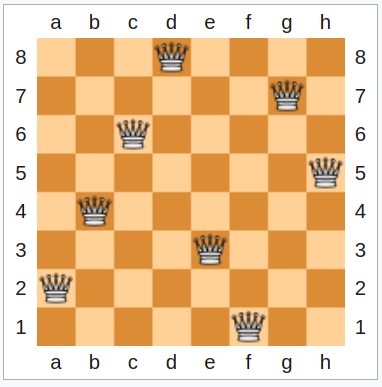
\includegraphics[scale=0.5]{fig/8queens.png}
    \centering
    \caption{Uma das soluções possíveis para o Problemas das Oito Rainhas.}
    \label{fig:myfig}
\end{figure}